You can find the code and everything else also on GitHub under the link \textit{https://github.com/awilsee/CSec}. Maybe more convenient for you.


\section{Warm It Up}
\lstinputlisting[caption=Code of task 1, label=lst:task1]{task1.py}

Firstly implemted the task using pycrypto lib. However this lib has a limit of 32 Byte for the key, so it's not usable for longer strings. Therefore implemented the \textit{xorfunc} by scratch. This functions will be used from the other tasks, as well. Realized the xorfunc with bytewise XOR with a for loop.\\


\section{Implement OTP}
\lstinputlisting[caption=Code of task 2, label=lst:task2]{task2.py}

For the One Time Pad (OTP) implemented reading and writing files in general. Additionally used the \textit{os.urandom}-function to generate the cipher key with the same length as the file. For encrypting and decrypting the key with the file the \textit{xorfunc} of \lstref{task1} is used.

\begin{lstlisting}
Input: "This is a textfile with some input over 32 Bytes.."
Hexadecimal output: "[0x6 0x6c 0x83 0x82 0x80 0x3e 0x8e 0x74 0x3a 0x8 0x50 0x98 0xe9 0xc4 0x65 0xa5 0xe 0xa2 0xba 0xcb 0xc1 0xa5 0xa7 0x86 0xa 0x1c 0xbb 0x21 0x94 0x1b 0x81 0x68 0x8c 0xad 0xf6 0xff 0x1e 0xdf 0x38 0xc8 0xa6 0x2b 0x1d 0x16 0x90 0xc1 0x5d 0x92 0xe5 0x43 0x3b]"
\end{lstlisting}


\section{Encrypt an Image Using OTP}
\lstinputlisting[caption=Code of task 3, label=lst:task3]{task3.py}

The function \textit{write\_bmp\_file} is used for writing the encrypted files with the original BMP-Header, so that it's possible to read it with an image viewer.

For encrytion of the BMP-File the function \textit{encryptBMPFile} was implemented which uses again the \textit{xorfunc} of \lstref{task1} and the previous mentioned one for saving.

With \textit{generateRndBMPFile} a BMP-File with random input will be created.\\

\begin{figure}[htp]
    \centering
    \caption{encrypted pictures}
	\subfloat[CP-Logo]{
        
\includegraphics[width=0.3\textwidth]{pics/cp-logo-enc3.png}
	}
	\subfloat[Mustang]{
        
\includegraphics[width=0.3\textwidth]{pics/mustang-enc3.png}
    }
	\subfloat[Random]{
        
\includegraphics[width=0.3\textwidth]{pics/random-enc3.png}
    }
\end{figure}

\textit{What do you observe?}\\
 You get a lot of random data where you can't see anything.\\
 
\textit{Are you able to derive any useful information about from either of the encrypted images? What are the causes for what you observe?}\\
You can't derive any useful information out of this images, because you XOR the data with different random keys which results in random data again.\\


\section{The Two-Time Pad}
\lstinputlisting[caption=Code of task 4, label=lst:task4]{task4.py}

\textit{EncryptBMPFile} of \lstref{task3} is used again for encryption of the BMP-Files with the same cipher key. Afterwards with function \textit{xorImages} both encrypted images are XOR together.

\begin{figure}[htp]
    \centering
    \caption{encrypted pictures}
	\subfloat[CP-Logo]{
        
\includegraphics[width=0.3\textwidth]{pics/cp-logo-enc4.png}
	}
	\subfloat[Mustang]{
        
\includegraphics[width=0.3\textwidth]{pics/mustang-enc4.png}
    }
	\subfloat[XOR a und b]{
        
\includegraphics[width=0.3\textwidth]{pics/xorPics.png}
        \label{fig:4xor}
    }
\end{figure}

\textit{Are you able to now derive any useful information about the original plaintexts from the resulting image? What are the causes for what you observe?}\\
Now you can see clearly recognize both pictures in figure \ref{fig:4xor}. The resulting picture is basically the first and second originally picture XOR together. Because if you XOR two times the same and with another XOR you get the same result as you only XOR the last one. And exactly that happend because we encrypted both pictures with the same key.\\


\section{Modes of Operation}
\lstinputlisting[caption=Code of task 5, label=lst:task5]{task5.py}

The first two functions are for adding the PKCS\#7 padding, so to fill up the 128-bits for the encryption. 

In the \textit{encrypt\_ecb} function is the operation mode of ECB implemented where each separate block of data will be encrypted by using the encrypt function of the cryptolib. The same cipher key is used for the whole program.

The decryption is basically the same as encryption in ECB-Mode except additionally the padding files will be removed. \\

In operation mode of CDC in each block of data the plaintext will be firstly XOR together either with INIT\_IV at the beginning or with the encrypted ciphertext block. After the XOR the encryption function of cryptolib is called.

The decryption is similiar. At first the block will be decrypted. Afterwards XOR together with INIT\_IV at the beginning or the previous ciphertext block.

To see that the own implementation of the encryption and decryption algorithm works correctly it was prooved with the cryptolib-function.


\begin{figure}[htp]
    \centering
    \caption{encrypted pictures in ECB}
	\subfloat[CP-Logo]{
        
\includegraphics[width=0.45\textwidth]{pics/cp-logo-enc-ecb.png}
	\label{fig:5ecba}
	}
	\subfloat[Mustang]{
        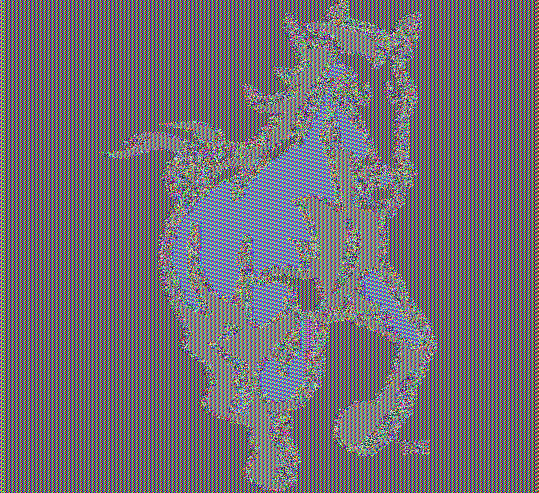
\includegraphics[width=0.45\textwidth]{pics/mustang-enc-ecb.png}
	\label{fig:5ecbb}
    }
\end{figure}


\begin{figure}[htp]
    \centering
    \caption{encrypted pictures in CBC}
	\subfloat[CP-Logo]{
        
\includegraphics[width=0.45\textwidth]{pics/cp-logo-enc-cbc.png}
	\label{fig:5cbca}
	}
	\subfloat[Mustang]{
        
\includegraphics[width=0.45\textwidth]{pics/mustang-enc-cbc.png}
	\label{fig:5cbcb}
    }
\end{figure}

\textit{What do you observe? Are you able to derive any useful information about from either of the encrypted images? What are the causes for what you observe?}\\
With ECB mode you can see in figure \ref{fig:5ecba} and \ref{fig:5ecbb} that you clearly can recognize what's in this picture. You don't have the image quality and colors but you definitely can see how it looks like. Well, the whole picture is encrypted with the exact same key and prozedure. So there will be some bits flipped which results in the change of color.\\
In CBC Mode as shown in figure \ref{fig:5cbca} and \ref{fig:5cbcb} it's random data, because you always take different data for the XOR function.

\section{The Limits of Confidentiality}
\lstinputlisting[caption=Code of task 6, label=lst:task6]{task6.py}

Firstly in the \textit{submit}-function the url is created with the payload. Afterwards the unwanted characters will be removed. For padding and encryption of this url text the functions of \lstref{task5} is used.

In the \textit{verify}-function the data will be decrypted with previous implemented function of \lstref{task5} and checked for the substring.

To modify the encrypted data in \textit{modify\_block}, the data will be firstly truncated into blocks of 128-bit. Now the ciphertext block before the actual plaintext block, where you wanna modify some bits, will be some bits flipped. You have to XOR the byte with the current plaintext sign and XOR it again with the sign you want because if you XOR with the same sign and afterwards with your own, only your own sing will be left after decryption.\\

\textit{Why was this attack possible? What would this scheme need in order to prevent such an attack?}\\
This attack is possible because it's always only dependent of the block before and the XOR function and there is no integrity of the data which is exactly used in this exploit.\\
A MAC or HMAC or an other authenticated encryption algorithm can be used to prevent this attack.\\


\section{Exploring Cryptographic Hash Functions}

\subsection{One-wayness}
\lstinputlisting[caption=Code of task 7, label=lst:task7, lastline=18]{task7.py}

\textit{What do you observe?}\\
The hash-function always creates completely different hexnumbers of 256-bits length. Despite you only change one bit in the string (Hamming Distance == 1) the hash is completely different.
\textit{How many of the bytes are different between the two digests?}\\
Mostly all of them.\\

\subsection{Preimage Resistance}
\lstinputlisting[caption=Code of task 7, label=lst:task7, firstline=22, lastline=33]{task7.py}

After the conversion of the byte-output to an integer the hash can be compared against the target numbers.\\

\begin{table}[h]
\begin{tabular}{|l|l|l|l|l|l|}
Target   & 0x0X & 0x00X & 0x000X & 0x0000X & 0x00000X \\
\hline
\#Inputs & 20   & 196   & 984    & 83765   & 114546  
\end{tabular}
\caption{results} \label{tab:7res}
\end{table}

\textit{What do you observe about the number of inputs required?}\\
As shown in table \ref{tab:7res} the number of required imputs increase exponentially, because more bytes have to be the same, where the probability is decreasing.\\


\subsection{Collision Resistance}
\lstinputlisting[caption=Code of task 7, label=lst:task7, firstline=35, lastline=107]{task7.py}

The task was to get the same sequence (several runs with different length of same sequence) of a hash twice with different input. Therefore new hashes will be generated and stored in a dictionary as long as two sequences of hashes matches together. To get the elapsed time a timestamp in line 15 in \lstref{task7} directly before the generation fo the hashes will be taken and after a hash match with another one and where the two inputs were different. The time function consider only the processing time, so not the sleeping time. This measurements was running on a Intel(R) Core(TM) i7-7500U CPU @ 2.70GHz.\\

For less memory usage and better performance only the sequence of the hash will be stored and the input number is limited to 20 Bytes.

For better statistics the whole prozedure was run 5 times with all different length from 8 bits till 50 bits in 2 bit steps and the average was calculated. And even with that I got to the limit of my computer with 16GB memory space and 52-bit sequence.\\

On figure \ref{fig:7num} and \ref{fig:7time} you can see that both are equal which also makes sense because the time is absolutely related to the number of inputs, as only the processing time was measured. So if you need more inputs you need more time because the computer can handle x inputs in a second, there is no variance. \\
In the graphs are the pointed lines the exact measurements and the red drawn through line is the average between them.\\
You can see that the time consumption respectively the needed number of input rises exponentially with the digest size.

\begin{figure}[h]
    \centering
    \caption{Plots of the \#inputs and time corresponding to digest size}
	\subfloat[digest with \#inputs]{
        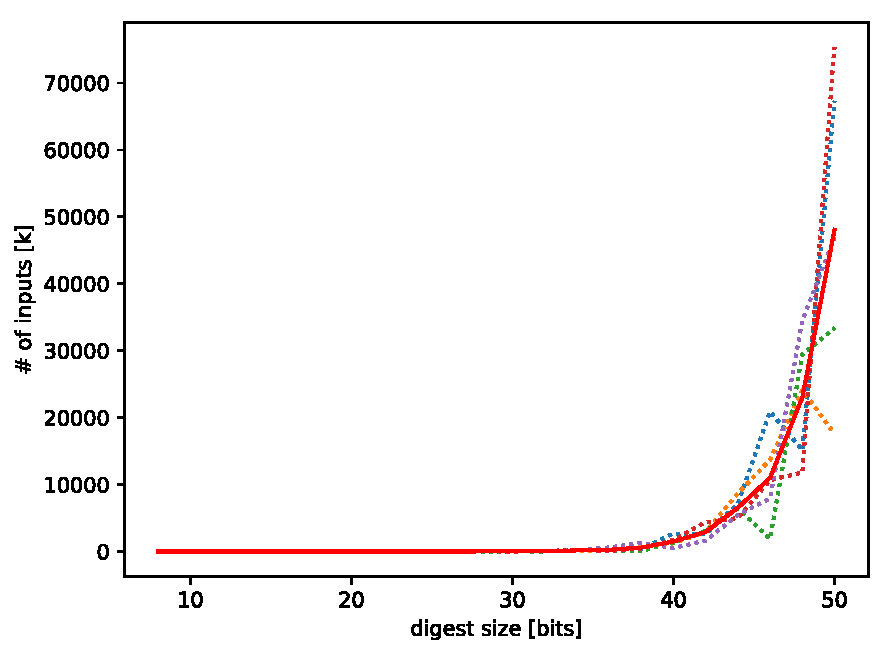
\includegraphics[width=0.5\textwidth]{pics/plot_num_input.pdf}
	\label{fig:7num}
	}
	\subfloat[digest with time]{
        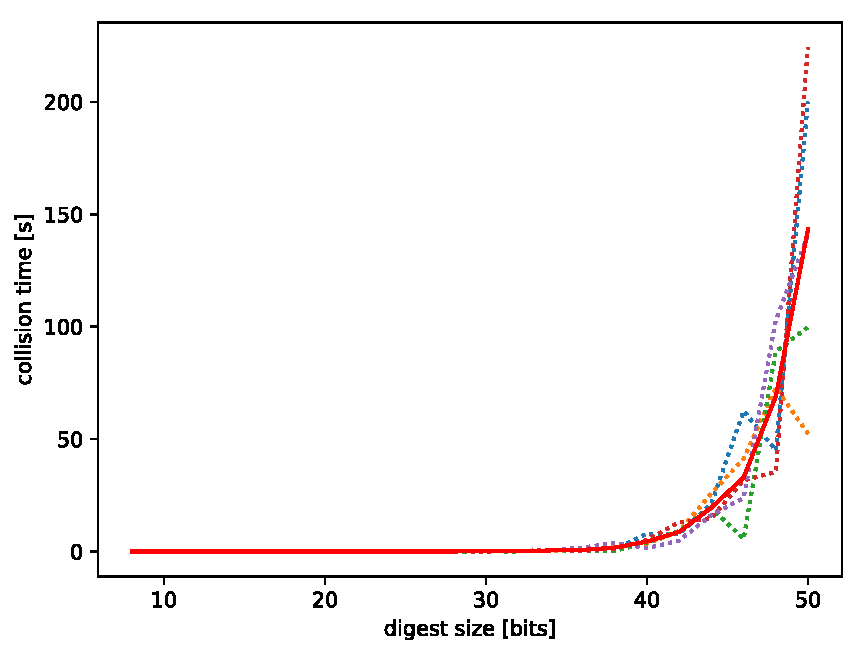
\includegraphics[width=0.5\textwidth]{pics/plot_time.pdf}
	\label{fig:7time}
    }
\end{figure}


\textit{What is the maximum number of files you would ever need to hash to find a collision on an n-bit digest?} \\
By the pigeon hole principle, we know that if we hash N+1 items, two of them are certain to have the same hash value.\\

\textit{Given the Birthday Bound, what is the expected number of hashes before a collision on an n-bit digest?}\\
With the Birthday Bound it would be $\sqrt{n}$.\\

\textit{Is this what you observed? Given the data you’ve collected, speculate on how long it might take to find a collision on the full 256-bit digest.} \\
Sure! It's obvious that a copmuter needs way longer the longer the same digest size is. The probability to find an equal hash decreases significantly.\\

\textit{Given an 8-bit digest, would you be able to break the one-way property (i.e. can you find any pre-image)?}\\
With the 256-bit hash function you will take forever. And even if you find a number which results in the same hash, it could be the wrong one because of the collisions.\\

\textit{Do you think this would be easier or harder (i.e. more or less work) than finding a collision? Why or why not?}\\
It's way more work and need way more time to calculate all posibilities. With the collisions and using the Birthday Bound you can look for any collision, doesn't matter with which hash. With the one-way you have to find exactly this one.